\documentclass[11pt,a4paper]{article}

% ===========================================================================
%  Manuscript for Methods in Ecology and Evolution
%  Auditing spatial information leakage in ecological prediction:
%  the spLeakage R package
% ===========================================================================

\usepackage[utf8]{inputenc}
\usepackage[T1]{fontenc}
\usepackage{lmodern}
\usepackage[a4paper,margin=2.5cm]{geometry}
\usepackage{amsmath,amssymb}
\usepackage{bm}
\usepackage{graphicx}
\usepackage{booktabs}
\usepackage{array}
\usepackage{caption}
\usepackage{xcolor}
\usepackage[hidelinks]{hyperref}
\usepackage{url}
\usepackage{natbib}
\usepackage{authblk}
\usepackage{setspace}
\usepackage{enumitem}
\usepackage{microtype}
\usepackage{tcolorbox}
\usepackage{listings}
\usepackage{lineno}

\bibliographystyle{apalike}
\tcbuselibrary{breakable,skins}

% --- boxed feature style (MEE-style Box) ---
\newtcolorbox{meebox}[1]{breakable, colback=black!3, colframe=black!55,
  fonttitle=\bfseries, title={#1}, boxrule=0.6pt, arc=2pt,
  left=6pt,right=6pt,top=5pt,bottom=5pt}

% --- R code style ---
\definecolor{codegray}{gray}{0.95}
\lstset{basicstyle=\ttfamily\footnotesize, backgroundcolor=\color{codegray},
  breaklines=true, frame=single, framesep=4pt, rulecolor=\color{black!25},
  keepspaces=true, columns=fullflexible, language=R, showstringspaces=false}

\newcommand{\SLI}{\mathrm{SLI}}
\newcommand{\SLIrho}{\SLI_{\rho}}
\newcommand{\SLId}{\SLI_{d}}
\newcommand{\EV}{\mathrm{EV}}
\newcommand{\E}{\mathbb{E}}
\newcommand{\cor}{\mathrm{cor}}

\title{\bfseries Auditing spatial information leakage in ecological prediction:
quantifying the optimism in map accuracy with the \texttt{spLeakage} R~package}

\author[1]{Olatunji Johnson}
\affil[1]{Department of Mathematics, University of Manchester, Manchester, UK.\\
Correspondence: \texttt{olatunji.johnson@manchester.ac.uk}}
\date{}

\begin{document}

\maketitle
\vspace{-2.2em}
\begin{center}\small Manuscript intended for \emph{Methods in Ecology and
Evolution} (Research Article / Application).\end{center}

\noindent\textbf{Running title:} Auditing spatial leakage in ecological maps

\medskip
\noindent\textbf{Word count} (main text, excl.\ abstract, boxes, references):
$\sim$6{,}000. \quad\textbf{Figures:} 4. \quad\textbf{Tables:} 2. \quad\textbf{Boxes:} 2.

\doublespacing
\linenumbers

% ===========================================================================
\section*{Abstract}
\begin{enumerate}[label=\arabic*.,leftmargin=1.6em,itemsep=3pt]
\item Ecologists increasingly turn field observations into wall-to-wall maps---of
species occurrence, abundance, biomass, traits and disease risk---and judge those
maps by an accuracy estimated through cross-validation (CV). When observations are
spatially autocorrelated, ordinary random CV places near-duplicate neighbours in
both training and test sets, so the model is graded on near-interpolation rather
than on the extrapolation the map is actually used for. Reported accuracy is then
\emph{optimistically biased}. Methods that \emph{prevent} this by building
spatially separated folds are well established, but no tool \emph{audits} the split
an analyst has already used (or a published result), or reports \emph{how much} the
accuracy is inflated.

\item The field is also divided: nearest-neighbour-matching CV treats random CV as
optimistic for clustered data, whereas design-based critics show that for
probability samples random CV is unbiased and spatial CV is \emph{pessimistic}.
Practitioners have had no way to tell which regime they are in.

\item We resolve both issues with one principle: spatial leakage and optimism are
well-defined only \emph{relative to a declared sampling design, estimand and
prediction target}. The same split can be leaking, correct, or pessimistic
according to those declarations---which dissolves the controversy (each side is
correct in a different setting) and makes optimism computable.

\item On this basis we introduce a \emph{signed} Spatial Leakage Index that audits
any split and maps where it leaks; give optimism a formal estimand (excess
explained variance under a Gaussian process) with a closed form and a Wasserstein
bound; and provide a refit-free, simulation-calibrated estimator of accuracy
inflation that flags when it is asked to extrapolate. All are implemented in the
open-source \texttt{spLeakage} R package, which \emph{audits rather than generates}
folds and interoperates with existing spatial-CV tools.

\item Validated against exact Gaussian-process algebra, the index is a
near-sufficient statistic for true optimism ($r=0.98$) and recovers the
\emph{direction} of bias that unsigned matching statistics cannot ($r=0.98$ vs
$-0.09$). Auditing 16 real spatial datasets, reported accuracy is optimistic in
\textbf{every} case (median 22\%), and optimism splits into an autocorrelation
component that spatial CV detects and a trend-extrapolation component it misses.
\texttt{spLeakage} gives ecologists a practical instrument to detect, quantify,
correct and pre-empt this overconfidence, complementing emerging reporting
standards for predictive models.
\end{enumerate}

\medskip
\noindent\textbf{Keywords:} area of applicability; cross-validation; map accuracy;
optimism bias; reproducibility; spatial autocorrelation; species distribution
models; validation.

% ===========================================================================
\section*{Plain language summary}
\noindent Ecologists routinely turn survey data into maps and report how accurate
those maps are. We show that the usual way of checking accuracy makes maps look
better than they are, because nearby survey points end up in both the ``learning''
and the ``testing'' data. We provide a free R package, \texttt{spLeakage}, that
takes a map-maker's existing analysis and reports how inflated the accuracy is,
where the problem is worst, and what to do about it---and we show that across many
real datasets reported accuracy is too high every time, by about a fifth on average.

% ===========================================================================
\section{Introduction}\label{sec:intro}

Predictive maps are now a primary product of quantitative ecology. Species
distribution models, abundance and biomass surfaces, habitat-suitability layers,
trait maps and disease-risk surfaces are all built by training a statistical or
machine-learning model on georeferenced observations and predicting across a
landscape \citep{araujo2019standards, zurell2020odmap}. The scientific and
management value of such a map hinges on one number: its estimated predictive
accuracy. If that number is wrong, decisions built on the map---reserve placement,
risk targeting, change detection---are miscalibrated in ways that are invisible to
the user.

For spatial data this number is systematically unreliable. Ecological observations
are spatially autocorrelated: nearby sites resemble one another. Under an ordinary
random train/test split, most test points have a training neighbour only a short
distance away, so the model is evaluated on a task close to \emph{interpolation}.
At deployment, however, the map must predict at locations far from any observation.
The reported error therefore understates the true error---it is
\emph{optimistically biased}---an instance of information \emph{leakage} from
training to test \citep{roberts2017crossvalidation, ploton2020spatial,
kattenborn2022spatially}. \citet{ploton2020spatial} showed that large-scale forest
biomass maps are far less accurate than reported once spatial structure is
respected; \citet{kattenborn2022spatially} documented the same inflation for
convolutional networks on vegetation imagery. Overconfidence in map accuracy is, in
short, a recognised and consequential problem in ecology.

\paragraph{What exists, and what is missing.}
A mature toolkit \emph{prevents} leakage by constructing spatially or
environmentally separated folds: spatial block CV
\citep{roberts2017crossvalidation, valavi2019blockcv}, buffered / spatial
leave-one-out CV \citep{lerest2014sloo, telford2009evaluation} and nearest-neighbour
distance matching CV \citep[NNDM/kNNDM;][]{mila2022nndm, linnenbrink2024knndm}, in
packages such as \texttt{CAST} \citep{meyer2024cast}, \texttt{blockCV}
\citep{valavi2019blockcv} and \texttt{spatialsample}. These are \emph{fold
generators}: they answer ``how should I cross-validate?''. None answers the question
an analyst who has already run a model---or a reader assessing a published map---
actually asks: \emph{how much does my split leak, and how inflated is the accuracy I
am about to report?} Reporting standards for distribution models now ask authors to
state how they validated \citep{araujo2019standards, zurell2020odmap}, but there has
been no instrument to \emph{audit} that validation and quantify its bias.

\paragraph{A live controversy.}
There is also genuine disagreement about what ``correct'' validation is.
\citet{mila2022nndm} and \citet{linnenbrink2024knndm} argue the CV geometry should
imitate the prediction geometry, making random CV optimistic for clustered data.
\citet{wadoux2021spatial} argue, from a design-based standpoint, that for a
\emph{probability sample} random validation is unbiased and spatial CV is
\emph{pessimistically} biased \citep[see also][]{debruin2022clustered}.
\textbf{Both are right, in different settings}---yet practitioners have no way to
identify their setting, and so no principled basis for choosing.

\paragraph{This paper.}
We argue the gap and the controversy share a cause and a cure. Spatial leakage and
optimism are not properties of a dataset or a split alone; they are defined only
relative to a declared sampling \emph{design}, \emph{estimand} and prediction
\emph{target} (Section~\ref{sec:framework}). Making these explicit dissolves the
controversy and renders optimism computable. We then contribute: (i) a \emph{signed}
Spatial Leakage Index that audits any split and maps where it leaks
(Section~\ref{sec:sli}); (ii) a formal estimand and theory for optimism, with a
closed form and a distribution-shift bound, presented for the general reader in
Box~1; (iii) a refit-free estimator of accuracy inflation that flags its own
extrapolation (Section~\ref{sec:optimism}); and (iv) design-aware guidance,
bias-corrected accuracy, and optimal validation-survey design
(Section~\ref{sec:recommend}). Everything is implemented in the open-source
\texttt{spLeakage} package (Section~\ref{sec:software}). Section~\ref{sec:examples}
validates the approach with exact algebra, a benchmark against NNDM, real-data
tests, a 16-dataset audit of field-wide overconfidence, and two real case studies---a
species distribution model and a disease-prevalence map---that show the audit
attributing leakage to different causes. Section~\ref{sec:discussion} gives practical
guidance (Box~2) and discusses scope and limitations.

% ===========================================================================
\section{A framework: leakage relative to design, estimand and
target}\label{sec:framework}

Our organising principle is:

\begin{quote}\itshape
``Spatial leakage'' and ``optimism'' are not properties of a dataset or a split in
isolation. They are well-defined only relative to a declared sampling
\textbf{design}, a declared \textbf{estimand}, and a declared prediction
\textbf{target}. The same split can be leaking, correct, or pessimistic depending on
these three declarations.
\end{quote}

\noindent The three declarations do distinct work.

\begin{description}[leftmargin=0pt,itemsep=3pt]
\item[Design.] Whether the data form a probability sample, a designed cluster
sample, or a convenience sample decides whether random validation is unbiased
\citep{wadoux2021spatial} or optimistic \citep{mila2022nndm}. Crucially,
design-basedness is a fact about \emph{how data were collected} and cannot be read
off the coordinates: a designed cluster sample and a convenience sample can produce
identical point patterns. Clustering statistics (Clark--Evans, Ripley's $K$) can
therefore only \emph{flag risk}; the design must be \emph{declared}.
\item[Estimand.] \emph{Mean map accuracy over a region} (a design-based quantity)
and \emph{conditional predictive skill at a location} (a model-based quantity) are
different questions; we never compare validation schemes across them.
\item[Target.] Predicting within the sampled footprint, mapping wall-to-wall, or
extrapolating to a new region imply different deployment geometries, and hence
different ``correct'' validation geometries.
\end{description}

This makes optimism well-posed: it is the gap between reported accuracy and the
accuracy under \emph{the validation that is correct for the declared
design~$\times$~estimand~$\times$~target}---not relative to any one method. For a
probability sample with a population-mean estimand, the correct baseline is random
validation, so a spatially blocked scheme registers as \emph{pessimism} (negative
optimism), exactly the design-based critique, now reported as such. Because the
declarations are inputs rather than inferences, the circularity that would otherwise
make optimism ill-posed disappears. This reconciliation is the conceptual core of
the paper; the index, the estimator and the recommender are its instruments.

% ===========================================================================
\section{The signed Spatial Leakage Index}\label{sec:sli}

For a split, let $g_{\text{obs}}(t)$ be the distance from each test point $t$ to its
nearest training point during CV, and $f_{\text{pred}}(p)$ the distance from each
deployment location $p$ to its nearest observation; distances are geodesic for
geographic coordinates and projected otherwise. Their empirical distribution
functions are $\widehat{G}_{\text{obs}}$ and $\widehat{G}_{\text{pred}}$. Leakage
means test points sit \emph{closer} to training data during CV than deployment
points will sit to the sample, i.e.\ $\widehat{G}_{\text{obs}}$ is shifted to
smaller distances.

\paragraph{Headline (dependence) form.} Because geographic distance is not the same
as statistical dependence, we convert distances to the fitted spatial correlation
$\rho(h)$ from the empirical variogram and define the mean \emph{retained spatial
information} under CV and at deployment,
\[
c_{\text{obs}}=\tfrac1n\textstyle\sum_t\rho\!\left(g_{\text{obs}}(t)\right),\qquad
c_{\text{pred}}=\tfrac1m\textstyle\sum_p\rho\!\left(f_{\text{pred}}(p)\right),
\]
\[
\boxed{\ \SLIrho=c_{\text{obs}}-c_{\text{pred}}\in[-1,1].\ }
\]
$\SLIrho$ is bounded, dimensionless and \emph{signed}: positive means CV retains more
spatial information than deployment has (optimistic leakage), negative means
pessimism, near zero means well matched. Under anisotropy or non-stationarity a
directional or local $\rho$ is used, so the index tracks dependence rather than raw
geometry. Box~1 shows that $\SLIrho$ is the leading term of true optimism, which is
what validates it.

\paragraph{Distance form and the bridge to NNDM.} A distance-scale companion
$\SLId$ is the signed area between the two distribution functions, normalised by the
variogram range. Its unsigned magnitude equals the NNDM/kNNDM Wasserstein statistic
$W$ when the curves do not cross, making the relationship to existing methods
explicit; a directionality ratio $\delta\in[-1,1]$ warns when the curves cross and a
single number should not be trusted.

\paragraph{Mapping the leak.} The per-observation contribution
$\ell(t)=\rho(g_{\text{obs}}(t))-c_{\text{pred}}$ sums to $\SLIrho$; mapping
$\ell(t)$ shows \emph{where} a split leaks and averaging within folds shows
\emph{which} folds leak. This decomposition of an arbitrary split---not just a
single summary number---is the substantive advance over a fold generator. Variogram
parameters are estimated, often from the very clustered data that leaks, so an
optional Monte-Carlo routine propagates that uncertainty into a confidence interval
on $\SLIrho$.

% --------------------- BOX 1: THEORY -------------------------------------
\begin{meebox}{Box 1.\quad What optimism \emph{is}, and why a geometric index
predicts it}
\small
Model the response as a Gaussian process plus noise:
$Y(s)=\mu+Z(s)+\varepsilon(s)$, with $\mathrm{Cov}(Z(s),Z(s'))=\sigma^2\rho(\lVert
s-s'\rVert)$ and $\varepsilon\sim N(0,\tau^2)$. Write the total variance
$V=\sigma^2+\tau^2$ and the \emph{signal proportion} $w=\sigma^2/V$. For optimal
(kriging) prediction, the error at a location is $V$ minus an \emph{explained
variance} term $\EV$ that grows the closer (more correlated) the location is to its
training data. Averaging over the test set (predicted from CV training folds) and
over the deployment target (predicted from the full sample), the constant $V$
cancels and

\vspace{-1.0em}
\[
\text{optimism}
=\underbrace{\tfrac1n\textstyle\sum_t \EV(t\mid \text{CV training})}_{\text{CV explains}}
-\underbrace{\tfrac1m\textstyle\sum_p \EV(p\mid \text{full sample})}_{\text{deployment explains}} .
\tag{B1.1}
\]

\vspace{-0.3em}
\noindent\textbf{Optimism is exactly the excess explained variance CV enjoys over
deployment} (B1.1 holds for any such process; it is positive when CV is ``easier''
than deployment and negative---pessimism---when harder). Keeping each point's
nearest neighbour, at distance $d$, the pointwise loss is
$L(d)\approx V[1-w^2\rho(d)^2]$, and (B1.1) becomes
\[
\text{optimism}\approx V\,w^2\Bigl(\E_t[\rho(g)^2]-\E_p[\rho(f)^2]\Bigr),
\tag{B1.2}
\]
i.e.\ (up to the scale $Vw^2$) a difference of mean retained correlation between CV
and deployment---\emph{the Spatial Leakage Index}. The theory therefore predicts
which quantities govern optimism (the correlation range and smoothness, the signal
proportion $w$, and the two nearest-neighbour-distance distributions) and explains
why a cheap geometric index can stand in for an expensive refit. Finally, because
$L$ is smooth and bounded, optimism is bounded by a Wasserstein-1 distance between
the CV and deployment distance distributions,
$|\text{optimism}|\le \lVert L'\rVert\, W_1$, connecting spatial leakage to
distribution-shift theory and giving $\SLId$ a rigorous interpretation as a bound.
\emph{Scope:} the single-neighbour form underestimates magnitude for dense data
(corrected by a $\approx1.6\times$ multi-neighbour factor); non-Gaussian responses
and non-kriging learners are handled empirically by the estimator below, for which
this theory gives the envelope.
\end{meebox}

% ===========================================================================
\section{From leakage to a number: estimating optimism}\label{sec:optimism}

A leakage score is abstract; ecologists want the consequence in their own currency:
\emph{``my reported accuracy is $X\%$ too high''}. \texttt{spLeakage} provides two
routes.

\paragraph{Refit route.} Re-evaluate the same model under the design-matched correct
scheme (e.g.\ spatial block CV for clustered data) and report the gap, using a metric
appropriate to the response---RMSE/MAE for continuous responses, and proper scoring
rules (Brier, log-loss, Poisson deviance) for occurrence, prevalence and count data,
so the optimism is meaningful for the binary and count responses common in ecology.
This is accurate but model-conditional and requires refitting.

\paragraph{Refit-free estimator.} A predictor maps the data and split geometry (range,
smoothness, signal proportion, sample size, clustering, the signed SLI, the declared
design and target) to expected optimism. It is calibrated once on a large simulation
study---shipped with the package---spanning Mat\'ern fields, random / clustered /
preferential sampling, Gaussian / Poisson / Binomial responses, and several learners
and targets, and returns an estimate with a calibrated (conformal) interval in
milliseconds, without refitting. Critically, the estimator carries its \emph{own}
area-of-applicability check \citep{meyer2021aoa}: when a dataset falls outside the
envelope it was trained on, it \emph{abstains} rather than extrapolate---a tool that
polices over-extrapolation must not commit it. When it abstains, the refit route
always applies.

% ===========================================================================
\section{Recommendation, correction and validation design}\label{sec:recommend}

\paragraph{Design-aware recommendation.} The framework becomes a decision aid that
elicits the estimand, then recommends over design~$\times$~target
(Table~\ref{tab:matrix}). Three rules keep it honest: the design is \emph{declared,
not inferred from geometry}; every recommendation is backed by a citation or a
simulation result; and guidance is conditional (``\emph{if} your estimand is $X$
under framework $Y$, \emph{then}\ldots''), surfacing the assumption rather than
quietly taking a side. It states plainly \emph{when spatial CV is not appropriate}.
A data-driven companion builds each candidate scheme on the user's own data and ranks
them by how closely each matches the declared deployment geometry.

\paragraph{Corrected accuracy.} A de-leaked estimator reports the accuracy an analyst
\emph{should} publish, with a bootstrap interval, and can translate a single
\emph{published} number into its corrected counterpart without the original model---
making the package usable for third-party review of existing maps.

\paragraph{Designing validation surveys.} Inverting the leakage logic, the package
allocates a budget of independent validation points to estimate true map accuracy
with minimum variance (distance-stratified Neyman allocation with inclusion weights),
turning leakage diagnosis into survey design.

\begin{table}[t]
\centering
\caption{Design~$\times$~target recommendation (after the estimand is declared). The
design is an elicited input; geometry only flags risk. Cells follow the cited
literature and our simulations (Section~\ref{sec:examples}).}
\label{tab:matrix}
\small
\begin{tabular}{p{3.3cm} p{2.9cm} p{2.9cm} p{3.1cm}}
\toprule
\textbf{Design $\backslash$ target} & \textbf{Interpolation} &
\textbf{Wall-to-wall map} & \textbf{New-region extrapolation}\\
\midrule
Probability / design-based & Random CV & Design-based estimator & Caution; AOA\\
Clustered / preferential & NNDM / buffered & NNDM / kNNDM & Block + AOA\\
Convenience / opportunistic & Buffered LOO & kNNDM & Block + AOA, flag risk\\
\bottomrule
\end{tabular}
\end{table}

% ===========================================================================
\section{The \texttt{spLeakage} package}\label{sec:software}

\texttt{spLeakage} is an R ($\ge 4.1$) package built on \texttt{sf}
\citep{pebesma2018sf}, with heavier adaptors (\texttt{rsample}, \texttt{mlr3},
\texttt{caret}, \texttt{blockCV}, \texttt{terra}, \texttt{gstat}) optional and
guarded at run time. It \emph{audits rather than generates} folds, interoperating
with the spatial-CV ecosystem. The core verbs are \texttt{detect\_leakage()} (the
signed SLI), \texttt{estimate\_optimism()} / \texttt{predict\_optimism()} (the two
optimism routes), \texttt{recommend\_validation()} / \texttt{rank\_cv\_schemes()}
(guidance), \texttt{deleak\_estimate()} (correction) and \texttt{design\_validation()}
(survey design), with channel-specific detectors for grouped/duplicated-location,
covariate-space, temporal, spatiotemporal and large-scale-trend leakage, each paired
with a fix. \texttt{audit\_workflow()} inspects an existing resampling object and
\texttt{report\_leakage()} produces a submission-ready scorecard. The package passes
\texttt{R CMD check} cleanly, ships three tutorials, and has a documentation website.

\begin{lstlisting}[caption={Auditing an existing species-distribution-model
validation in five lines.},captionpos=b]
library(spLeakage)
tgt <- prediction_target(grid = pred_grid, type = "grid")   # where the map is used
lk  <- detect_leakage(occ, split = my_folds, target = tgt,  # signed leakage index
                      response = "presence", n_boot = 300)
lk; plot(lk)                                                 # score, CI, ECDFs, map
predict_optimism(lk)                                         # "% accuracy inflated"
recommend_validation(occ, estimand = "prediction",          # what to do instead
                     design = "clustered", target = "grid")
\end{lstlisting}

% ===========================================================================
\section{Worked examples and validation}\label{sec:examples}

We validate each claim in turn; scripts to reproduce every result ship with the
package.

\subsection{The index is a near-sufficient statistic for optimism}

Across 192 Gaussian-process configurations, with explained variance computed exactly
from covariance algebra (Box~1), the unsigned closed form (B1.2) tracks true optimism
at $r=0.975$, and the package's $\SLIrho$ at $r=0.976$---explaining $\approx 95\%$ of
the variance in true optimism (Table~\ref{tab:theory}; Fig.~\ref{fig:sli}). The
Wasserstein bound holds in $100\%$ of configurations for the quantity it governs.

\begin{table}[t]
\centering
\caption{Exact Gaussian-process validation of the theory in Box~1 (192
configurations).}
\label{tab:theory}
\small
\begin{tabular}{p{9.2cm} c}
\toprule
Claim & Result\\
\midrule
Closed form (B1.2) predicts exact optimism & $r=0.975$\\
$\SLIrho$ is a near-sufficient statistic for optimism & $r=0.976$\\
Wasserstein bound holds (single-neighbour optimism) & $100\%$\\
Multi-neighbour amplification (exact / single-neighbour) & median $1.56$\\
\bottomrule
\end{tabular}
\end{table}

\subsection{Signed leakage recovers what matching statistics cannot}

The natural question---``is this just NNDM's $W$?''---is answered against exact
optimism over 288 configurations, $64\%$ of which are \emph{pessimistic} (the
design-based regime). The signed $\SLIrho$ predicts \emph{signed} optimism at
$r=0.977$; the unsigned $W$ at $r=-0.090$ (Table~\ref{tab:benchmark}). $W$ cannot
sign the bias by construction, so a large $W$ leaves an analyst unsure whether to
trust their accuracy more or less; the signed index recovers the direction in $97\%$
of cases and beats $W$ on magnitude because it carries the signal proportion that
scales optimism. NNDM solves a fold-construction problem; \texttt{spLeakage} solves a
diagnosis problem.

\begin{table}[t]
\centering
\caption{Predicting exact optimism from the signed SLI versus NNDM's unsigned $W$
(288 configurations).}
\label{tab:benchmark}
\small
\begin{tabular}{l c c}
\toprule
Task & signed $\SLIrho$ & NNDM $W$ (unsigned)\\
\midrule
Predict \emph{signed} optimism & $r=+0.977$ & $r=-0.090$\\
Predict magnitude & $r=0.955$ & $r=0.672$\\
Direction (sign) agreement & $97\%$ & silent by construction\\
\bottomrule
\end{tabular}
\end{table}

\subsection{The estimator generalises, and reconciles the controversy}

On a study of 1000 configurations held out by configuration, the refit-free estimator
attains $R^2\approx0.76$, places $97\%$ of queries inside its area of applicability,
and its $90\%$ intervals cover at $\approx94\%$ (Fig.~\ref{fig:calibration}). The
design effect that reconciles the debate reproduces in the data: clustered and
preferential sampling shift random CV toward optimism (the Mil\`a regime), while for
well-covered targets with probability-like samples random CV is unbiased or slightly
pessimistic (the design-based regime); the ordering is robust (Fig.~\ref{fig:design}).

\begin{figure}[t]
\centering
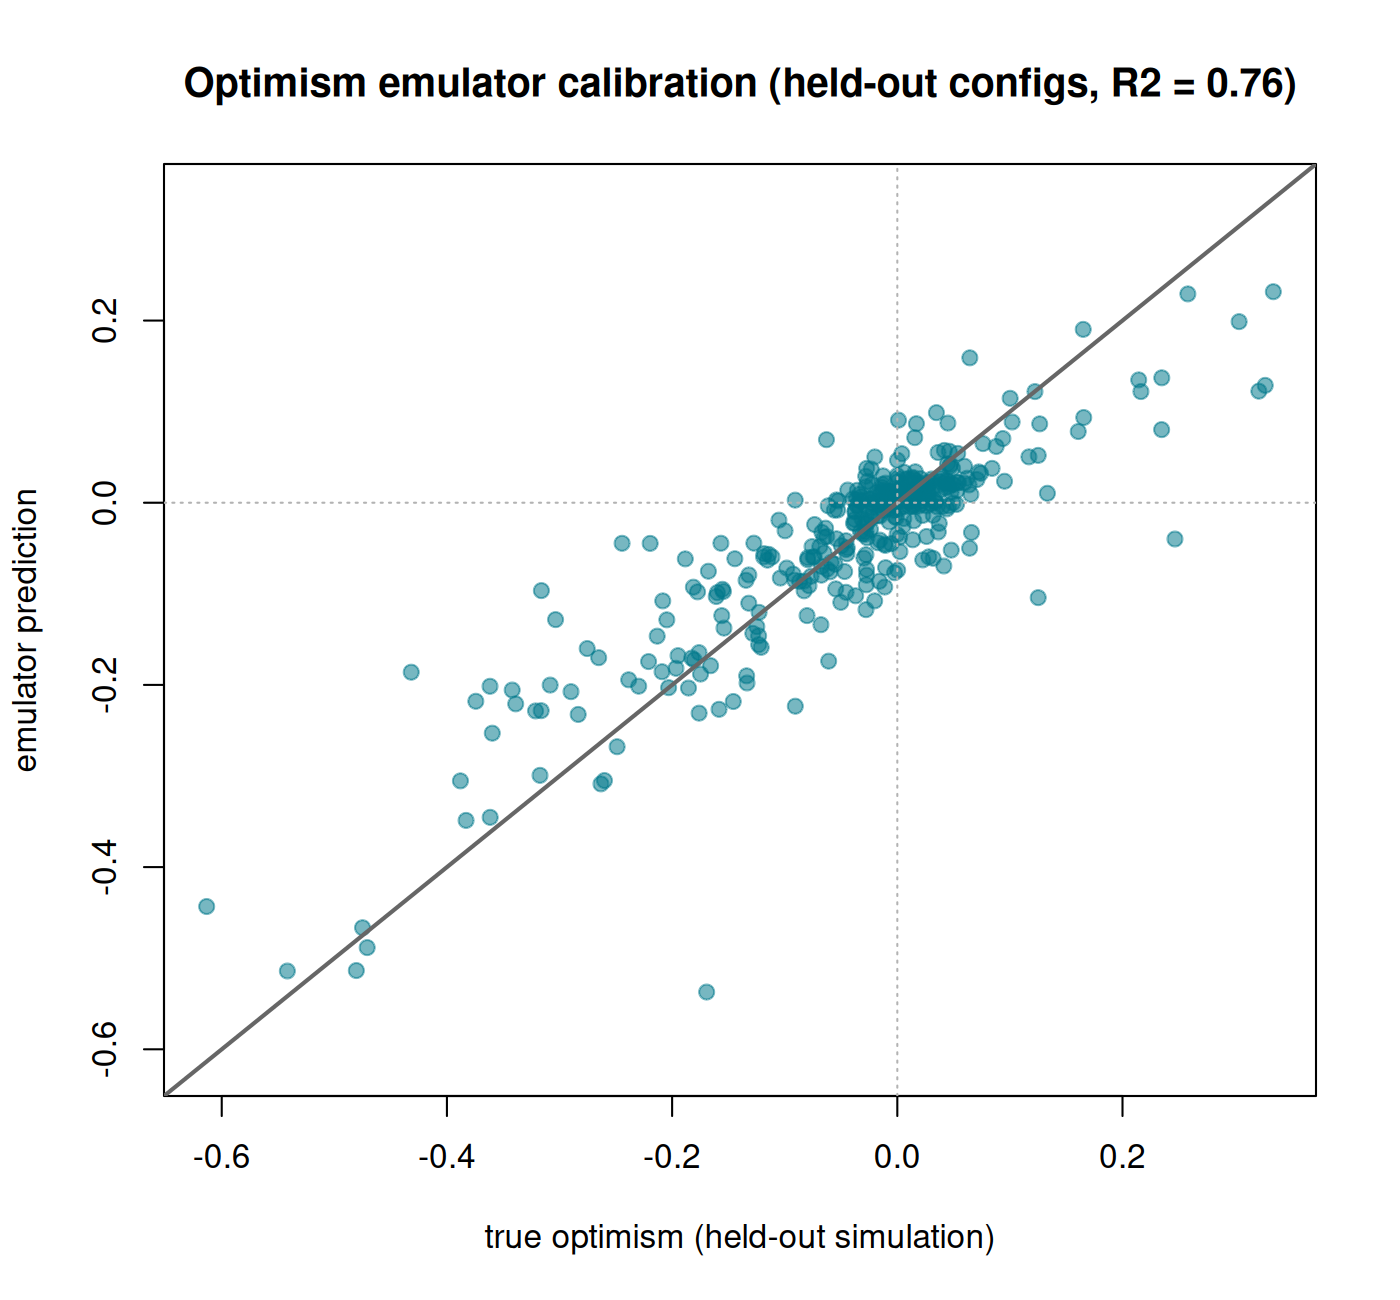
\includegraphics[width=0.72\textwidth]{figures/F1_calibration.png}
\caption{Out-of-sample calibration of the refit-free optimism estimator (held out by
configuration): predicted versus true optimism with conformal intervals; $R^2\approx
0.76$, interval coverage $\approx94\%$, $97\%$ of queries within the area of
applicability.}
\label{fig:calibration}
\end{figure}

\begin{figure}[t]
\centering
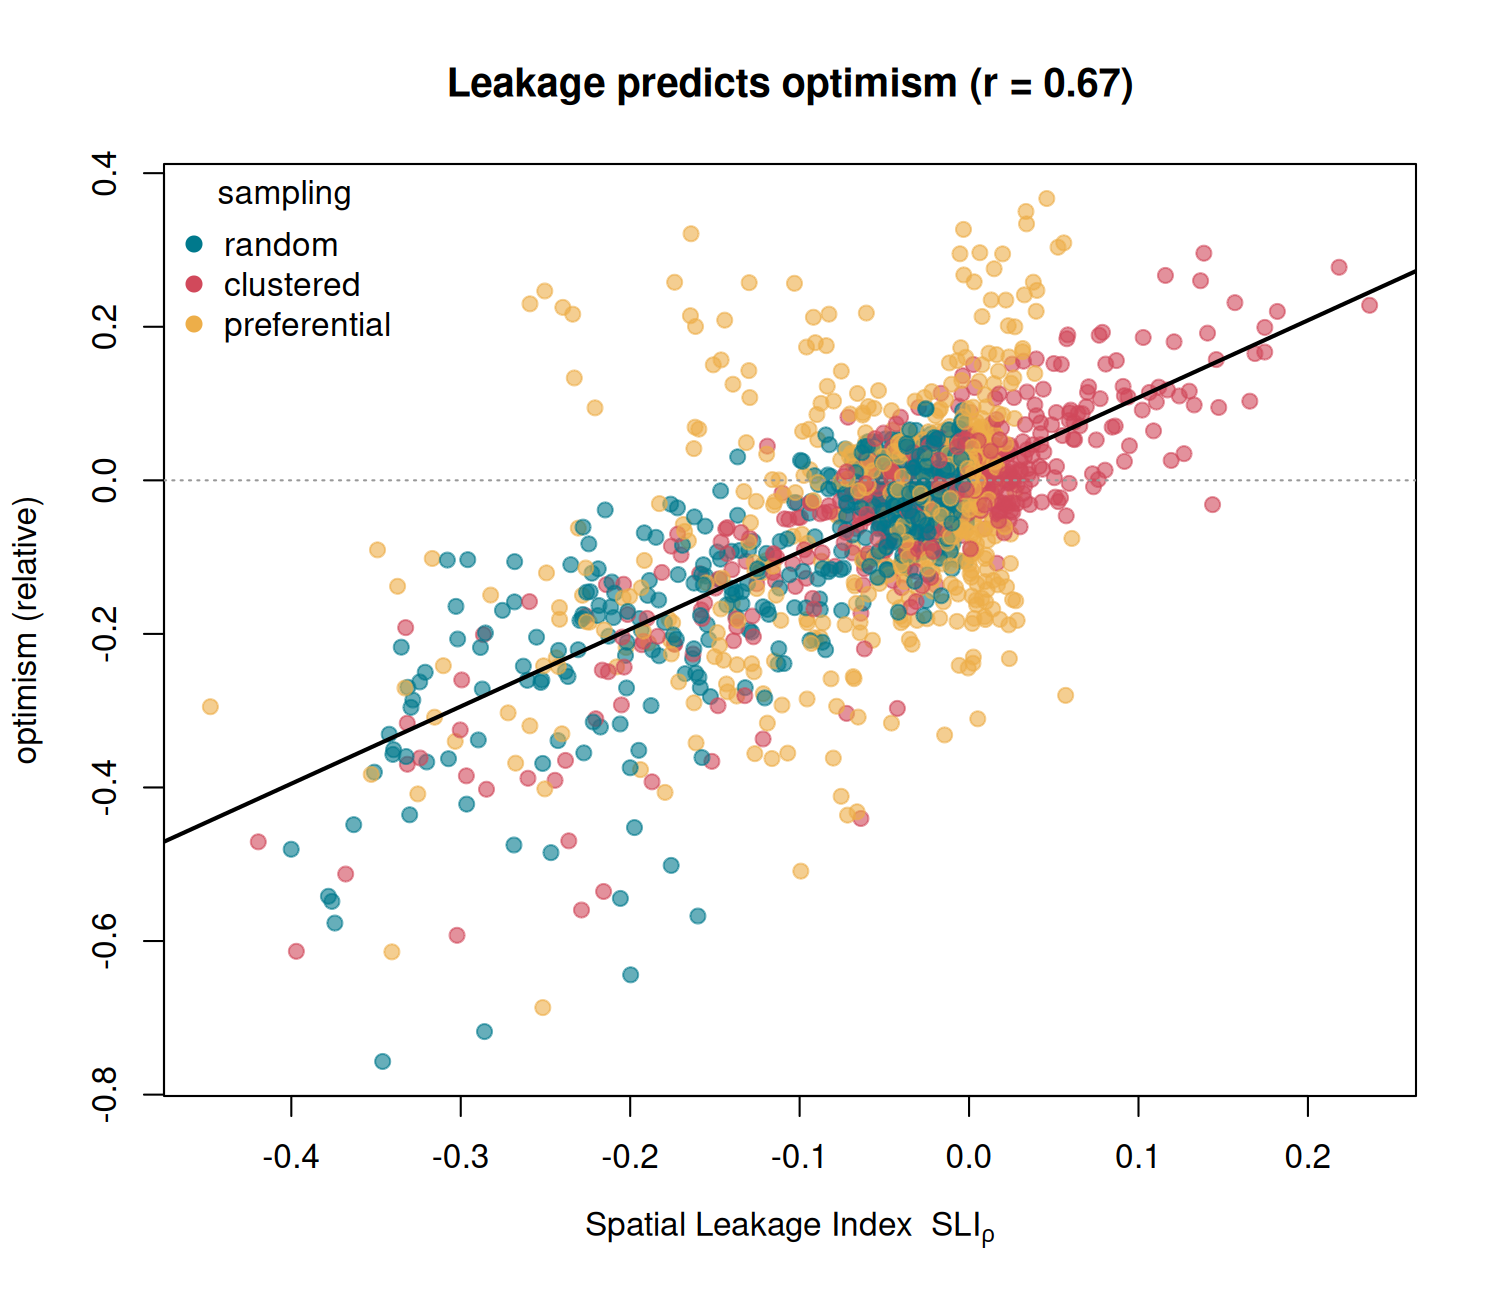
\includegraphics[width=0.72\textwidth]{figures/F2_sli_vs_optimism.png}
\caption{The Spatial Leakage Index tracks true optimism across the simulation grid
(empirical $\cor=0.67$; $r=0.98$ against exact optimism), the empirical counterpart
of Box~1, eq.~(B1.2).}
\label{fig:sli}
\end{figure}

\begin{figure}[t]
\centering
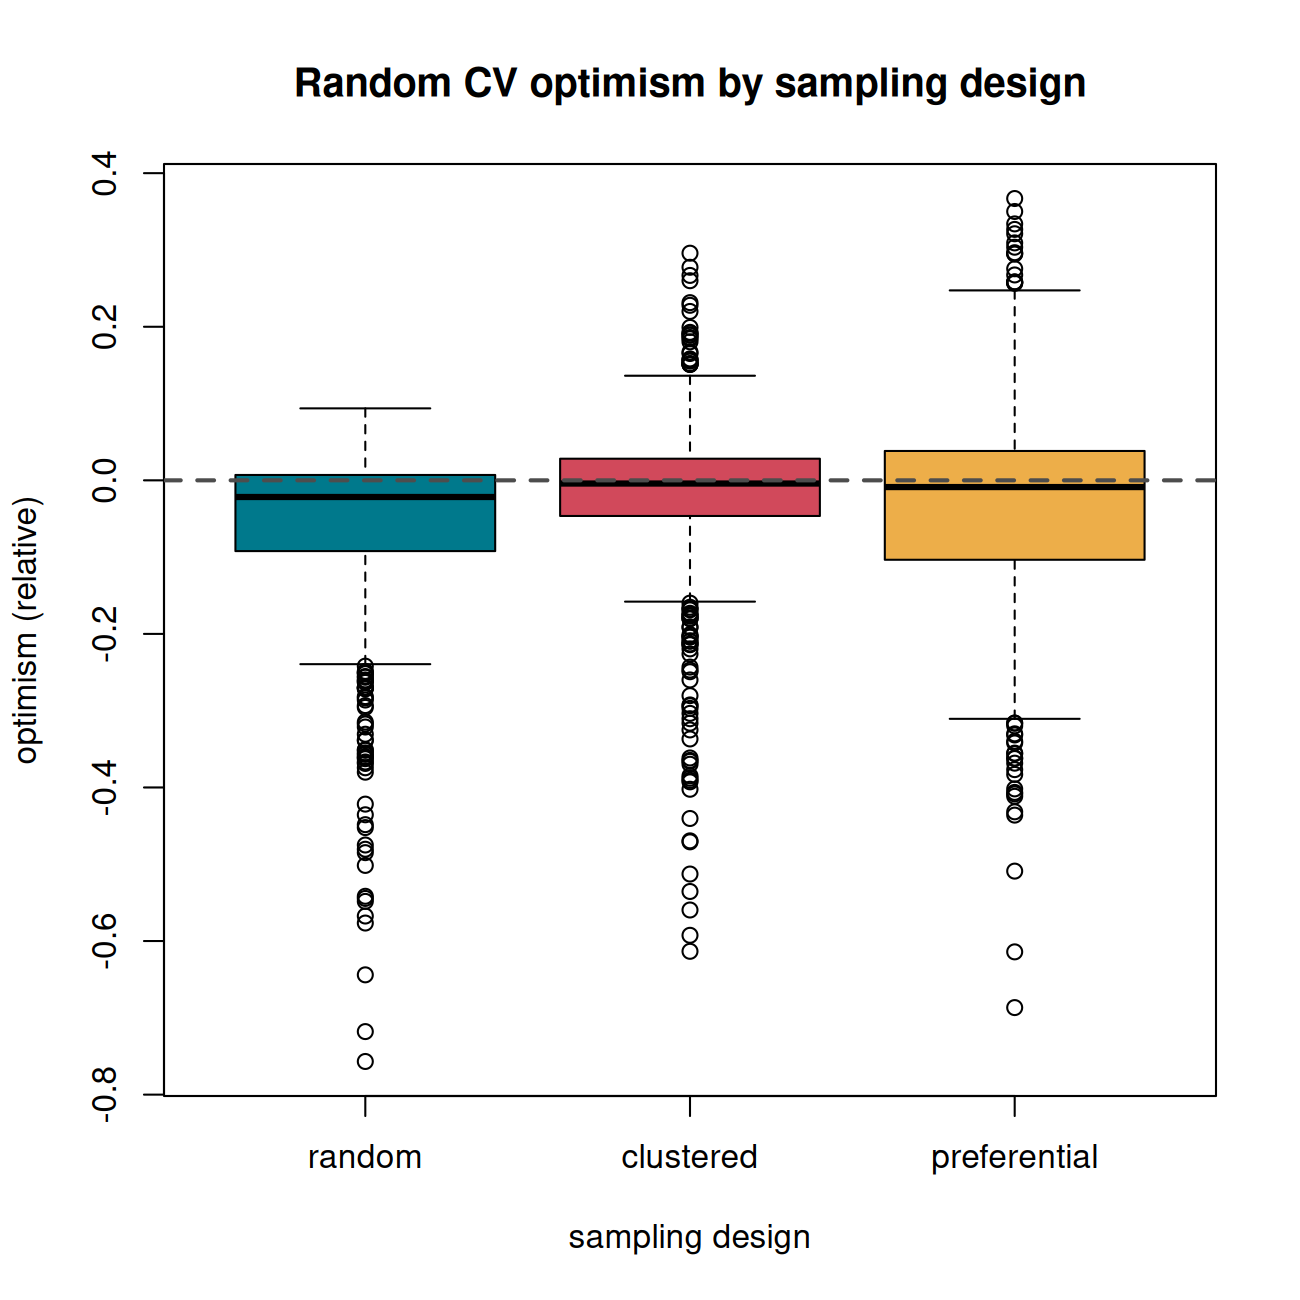
\includegraphics[width=0.72\textwidth]{figures/F3_design.png}
\caption{Reconciling the controversy. The optimism of random CV depends on sampling
design and target: clustered/preferential designs push random CV toward optimism;
probability-like samples on well-covered targets make it unbiased or slightly
pessimistic. Both are cells of one framework, not contradictory claims.}
\label{fig:design}
\end{figure}

\subsection{Real fields: the problem is real and large}

On three real spatial fields evaluated against genuinely independent held-out data
(240 replicates), naive random CV understates true error by a median of $36\%$ under
extrapolation. The target-aware SLI separates extrapolation from interpolation
deployments as real optimism does ($\cor=0.52$), and the de-leaked estimate recovers
up to $89\%$ of the true independent error---without ever seeing the held-out data.

\subsection{How overconfident is ecological mapping? A 16-dataset audit}

Using \texttt{spLeakage} as the instrument on 16 real spatial response variables
(soil chemistry, heavy metals, rainfall, elevation, ozone and disease prevalence),
with real optimism measured by spatial region-holdout, reported accuracy is
optimistic in \textbf{every} dataset, with a median of $22\%$ (interquartile range
$17$--$34\%$) and more than $20\%$ in two-thirds (Fig.~\ref{fig:metaaudit}).

The audit also reveals that optimism has \emph{two} components. The autocorrelation
component is what the SLI and NNDM detect. But the smooth, trend-dominated fields
(rainfall, elevation) show the \emph{largest} optimism ($40$--$54\%$) with almost no
short-range leakage signal: their error is the model's inability to extrapolate a
large-scale \emph{trend}, to which autocorrelation-based diagnostics are blind. A
trend-strength feature recovers exactly this missed signal ($r=+0.75$). Field-wide
overconfidence is therefore a two-channel phenomenon, and the $22\%$ median is a
\emph{lower bound} on what autocorrelation-aware tooling alone would catch.

\begin{figure}[t]
\centering
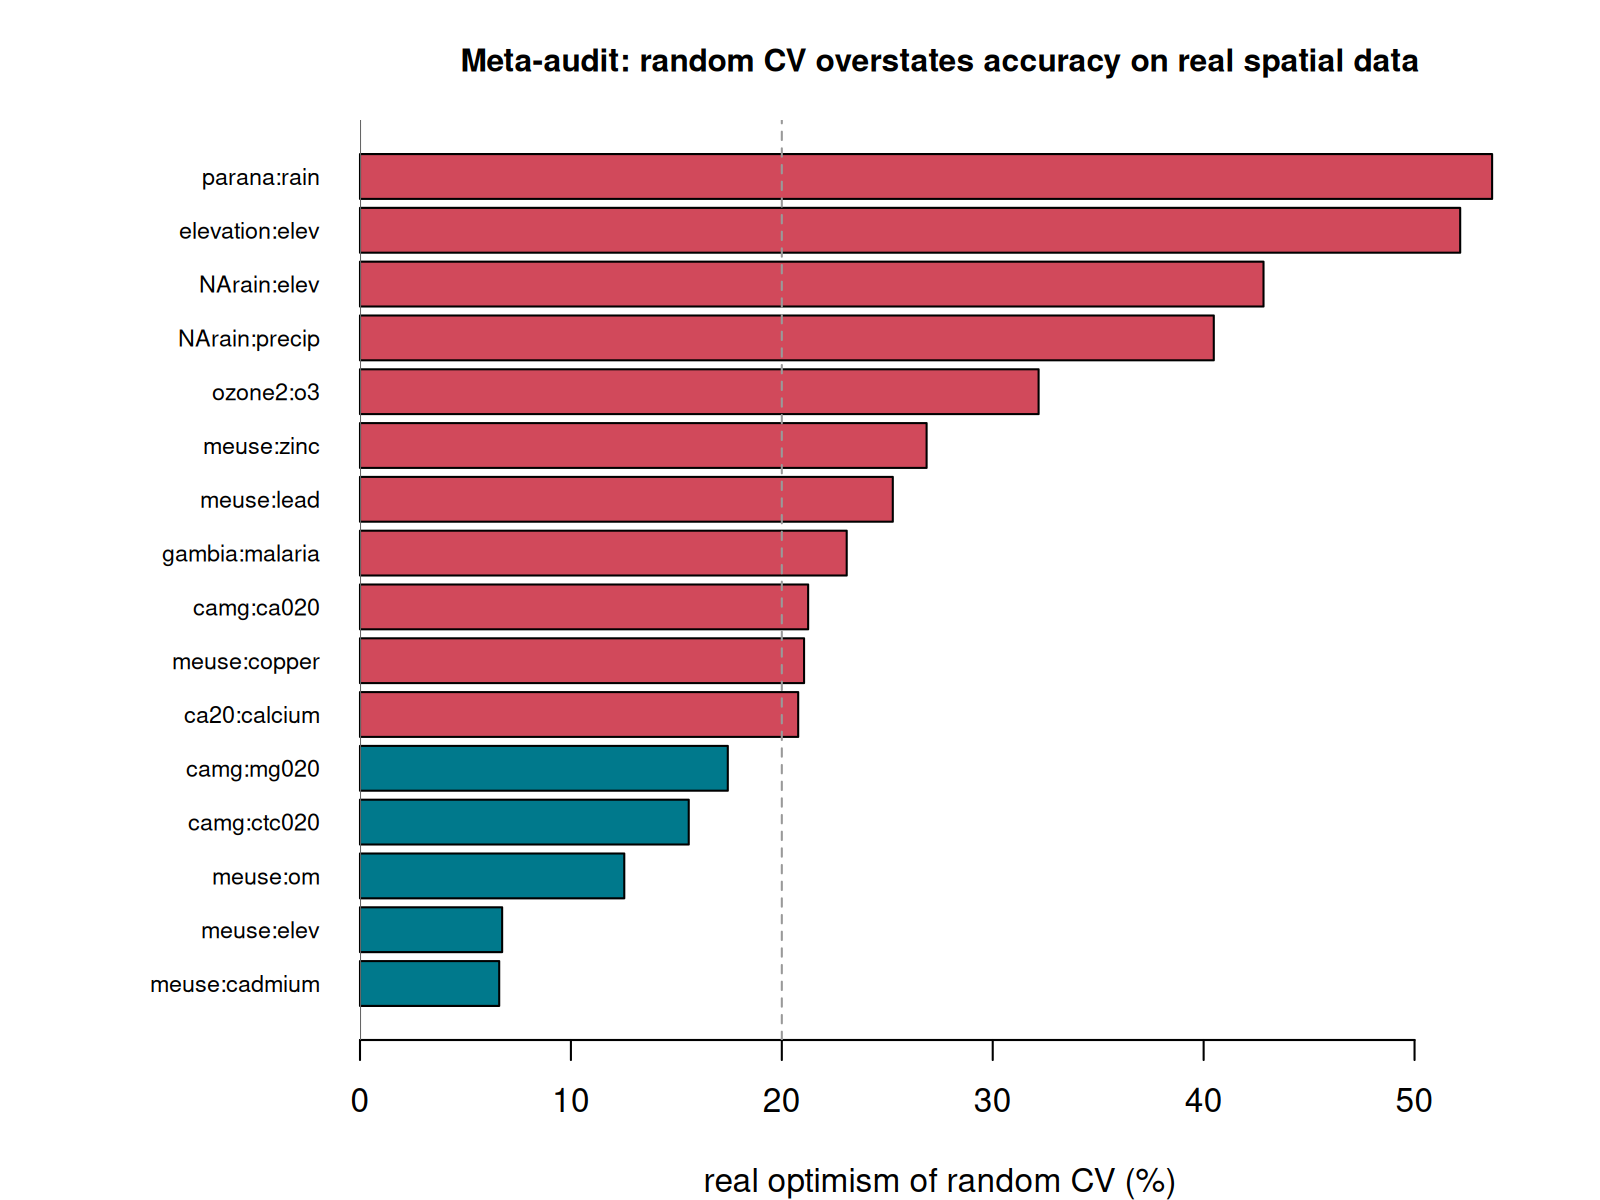
\includegraphics[width=0.76\textwidth]{figures/F4_meta_audit.png}
\caption{Auditing 16 real spatial datasets. Naive random CV is optimistic for every
one (median $22\%$). The trend-dominated fields show the largest optimism yet the
weakest short-range leakage---the second, trend-extrapolation channel.}
\label{fig:metaaudit}
\end{figure}

\subsection{Case studies: two real maps, two leakage signatures}

We close with two real applications that a single audit must be able to tell apart:
a species distribution model whose optimism is genuine spatial autocorrelation, and a
disease-prevalence map whose apparent leakage is in fact a survey-design artefact.
Together they show \texttt{spLeakage} attributing leakage to the \emph{right} cause.

\paragraph{Lead case: a species distribution model.}
We audit a presence/absence SDM built on the south-east Australia dataset of
\citet{valavi2019blockcv} (500 records; 243 presence; four bioclim covariates),
predicting a wall-to-wall habitat-suitability map. An ecologist's default---a random
10-fold split validated with the Brier score---returns an optimistic split:
$\SLIrho=+0.10$ (90\% CI $+0.07,+0.14$), and the Brier score is \textbf{$42\%$ too
good} relative to the design-matched block scheme. Two further channels sharpen the
diagnosis. The covariate-space audit shows the map \emph{extrapolates} the bioclim
predictors well beyond where the model was tested (deployment covariate-space reach
$3.73$ vs test reach $1.04$; signed feature leakage $+2.7$)---a concrete
area-of-applicability warning for the suitability surface. Meanwhile the
grouped-location channel finds \emph{no} co-located duplicates, so this optimism is
genuine autocorrelation, not a sampling artefact. Ranking candidate schemes on the
data reproduces the paper's central nuance: random CV is optimistic ($+0.10$),
buffered CV is \emph{over-corrected into pessimism} ($-0.22$), and block CV best
matches deployment ($-0.004$)---a distinction no static decision table provides.

\paragraph{Second case: mapping malaria prevalence.}
On geolocated \emph{Plasmodium falciparum} prevalence surveys in Nigeria
\citep{weiss2019mapping} ($n=66$), a naive random split gives $\SLIrho=+0.212$ despite
a near-zero variogram signal---an apparent paradox the package resolves: the
grouped-location channel attributes $21.2\%$ of test points to leakage through
\emph{co-located repeat surveys}, deduplication collapses $\SLIrho$ to $+0.006$, and
the grouped fix removes it entirely. The refit-free estimator correctly
\emph{abstained} ($n$ below its training envelope), demonstrating the
area-of-applicability guard on real data. Where the SDM's leakage was real
autocorrelation, here it is a survey-design artefact---routine in ecological and
epidemiological data with revisited sites (fixed plots, transect re-surveys,
sentinel stations). The same multi-channel audit reaches opposite, correct verdicts
in the two cases.

% ===========================================================================
\section{Discussion}\label{sec:discussion}

\paragraph{A settled controversy and a practical workflow.} The disagreement over
spatial CV is not a conflict of facts but of settings. Once design, estimand and
target are declared, optimism is a well-posed, signed quantity, and the data decide
which prescription applies. \texttt{spLeakage} reports the setting and prescribes
accordingly, conditionally rather than dogmatically (Box~2). It complements rather
than competes with fold generators (\texttt{CAST}, \texttt{blockCV},
\texttt{spatialsample}) and with reporting standards \citep{araujo2019standards,
zurell2020odmap}: where those ask authors to \emph{describe} their validation, this
lets authors and reviewers \emph{audit} it.

\paragraph{Scope and limitations.} The theory in Box~1 is a Gaussian backbone:
the single-neighbour form underestimates magnitude for dense data (correctable by a
multi-neighbour factor), and non-Gaussian responses and non-kriging learners are
handled empirically by the estimator, for which the theory gives the envelope. The
estimator is honest about its own extrapolation and abstains when out of range. The
most important open finding is the trend-extrapolation channel that all
autocorrelation-based diagnostics miss; it is now flagged by a trend-strength feature
but deserves a fully trend- and covariate-aware optimism model. Finally,
design-basedness must be elicited: no geometric test can certify a probability
sample, so the recommender is decision \emph{support}, not automation.

\paragraph{Outlook.} The distribution-shift view (Box~1) points toward model-agnostic
optimism bounds beyond the Gaussian case, and coupling the autocorrelation and trend
channels into one estimator is a clear next step. We hope the package becomes a
routine step between fitting an ecological map and reporting its accuracy.

% --------------------- BOX 2: GUIDANCE -----------------------------------
\begin{meebox}{Box 2.\quad A checklist for auditing your own map validation}
\small
\begin{enumerate}[leftmargin=1.4em,itemsep=2pt]
\item \textbf{Declare the deployment target.} Are you interpolating within the
sampled area, mapping wall-to-wall, or extrapolating to a new region?
(\texttt{prediction\_target()}.)
\item \textbf{Declare the sampling design and estimand.} Is it a probability sample
or opportunistic data? Do you want mean map accuracy or skill at a location? These
are facts you know and the coordinates do not.
\item \textbf{Audit the split.} Run \texttt{detect\_leakage()}; read the
\emph{signed} index and its interval, and \texttt{plot()} where it leaks.
\item \textbf{Check other channels.} Revisited sites, covariate-space extrapolation,
time, and large-scale trend (\texttt{audit\_workflow()}).
\item \textbf{Quantify and correct.} Get the \% inflation
(\texttt{predict\_optimism()} / \texttt{estimate\_optimism()}) and report the
de-leaked accuracy (\texttt{deleak\_estimate()}).
\item \textbf{Act on the recommendation.} Use \texttt{recommend\_validation()} /
\texttt{rank\_cv\_schemes()}---and heed it when it says spatial CV is \emph{not}
appropriate.
\end{enumerate}
\end{meebox}

% ===========================================================================
\section*{Acknowledgements}
The author thanks the developers of the spatial cross-validation ecosystem
(\texttt{CAST}, \texttt{blockCV}, \texttt{spatialsample}, \texttt{mlr3spatiotempcv})
whose work this package builds upon and audits.

\section*{Conflict of interest}
The author declares no conflict of interest.

\section*{Author contributions}
OJ conceived the study, developed the methods and software, performed the analyses
and wrote the manuscript.

\section*{Data availability and reproducibility}
The \texttt{spLeakage} package and all analysis scripts that reproduce the results
are openly available at \url{https://github.com/olatunjijohnson/spLeakage} (MIT
licence), with documentation at \url{https://olatunjijohnson.github.io/spLeakage/}.
All datasets are public (the south-east Australia presence/absence SDM data and
bioclim covariates via \texttt{blockCV}; Malaria Atlas Project via
\texttt{malariaAtlas}; \texttt{meuse}, \texttt{ca20}, Paran\'a and the remaining
audit fields via \texttt{sp}, \texttt{geoR} and \texttt{gstat}). Code archival on
Zenodo with a DOI
will accompany acceptance.

\bibliography{refs}

\end{document}
